\section{Contexte \& Démarche}
\subsection{Contexte}
Le projet se déroule dans une équipe historiquement d'intégration. Ce n'est pas une équipe de développement.
La fonction de l'équipe évolue suite au mouvement "devops", maintenant ils soutiennent des équipes de développement sur l'intégration.
On a une structure transverse, les membres sont sur des projets différents.

Le projet est cadré par mon encadrant de stage qui désigne les objectifs du projet.
Pour le réaliser, je suis accompagné d'un référent technique.
Le travail se fait en autonomie, mais j'ai l'appui de toute l'équipe.

\subsection{Démarche}
Dans cette équipe, on applique un "Kanban"(lexique. \ref{lexi:kanban}) pour l'organisation des travaux.
Comme sur la figure (fig. \ref{fig:kanban}), chaque membre dispose d'une ligne sur le tableau et chaque ligne est découpé en trois parties: "TODO", "EN-COUR" et "DONE" qui correspondant aux tâches à faire, tâche en train de faire et tâches réalisés.
Les espaces laissés à gauche sont pour des idées qu'on va pêut-être planifier un jour.

\begin{figure}[ht]
\centering
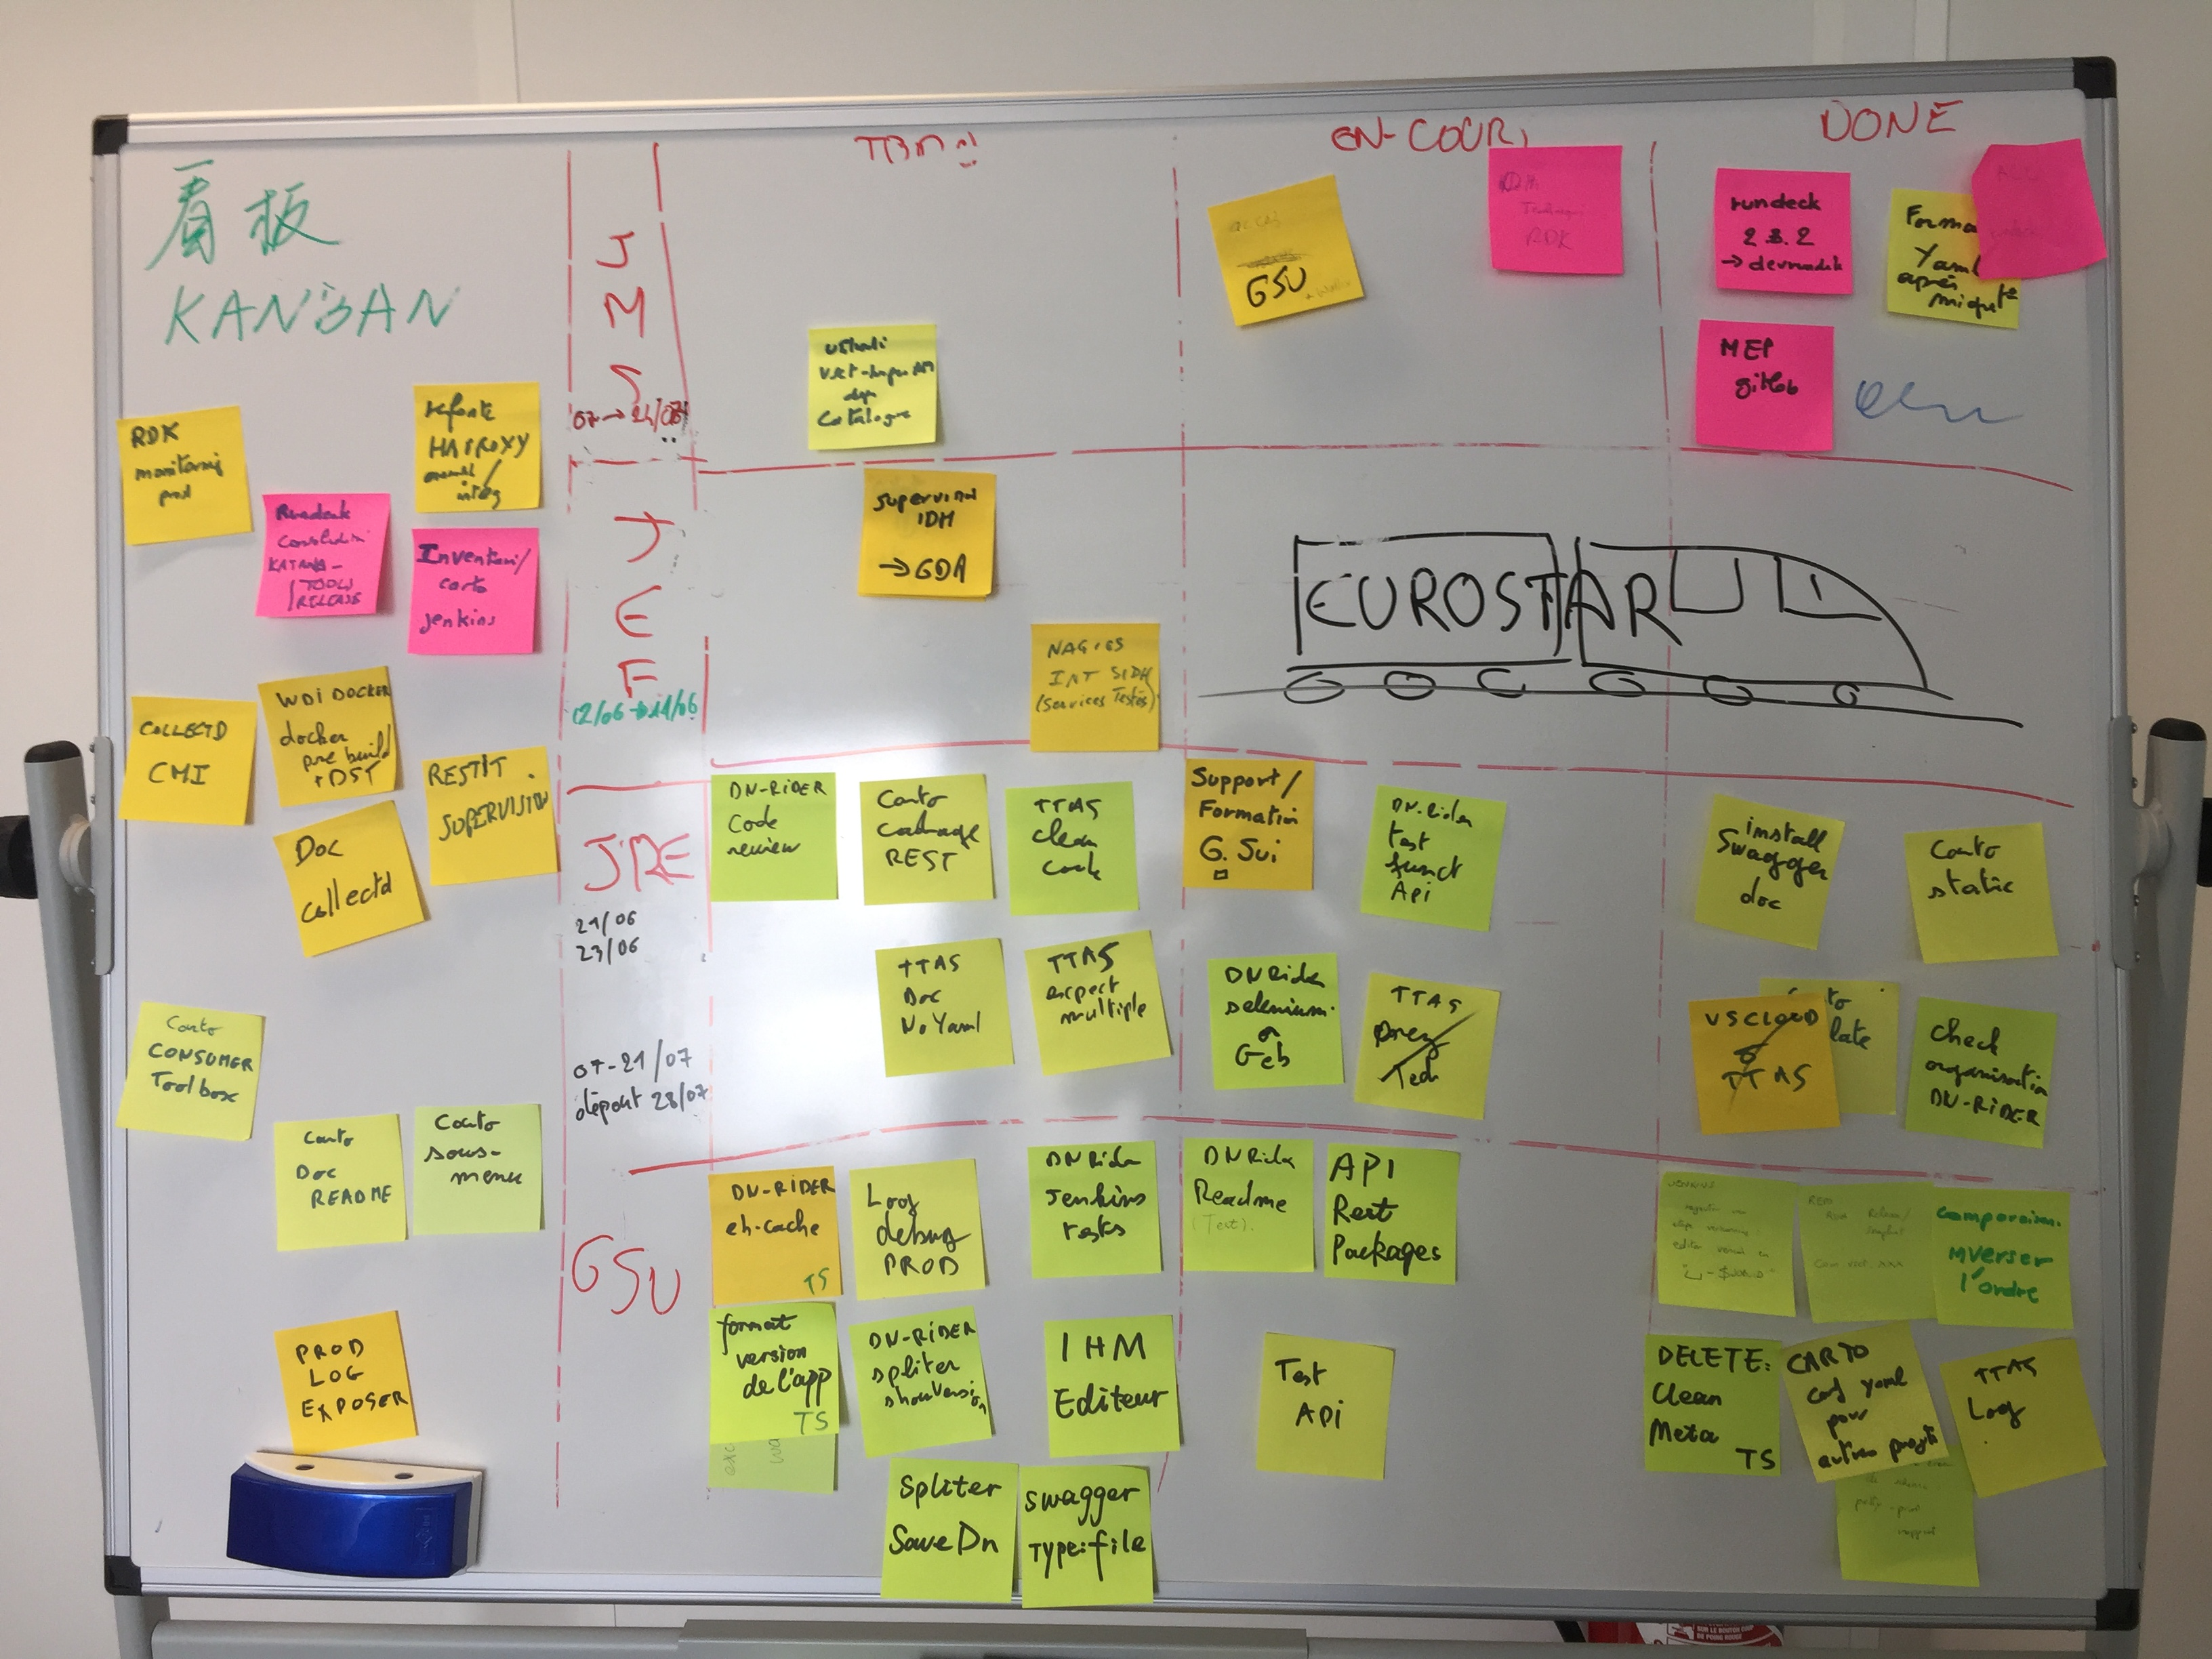
\includegraphics[width=0.7\textwidth]{kanban}
\caption{Kanban}
\label{fig:kanban}
\end{figure}

Les tâches sont representées par des "post-it" et des elements du backlog (fig.\ref{fig:backlog}),
Certaines cartes sont marquées "TS" (Technic Story) dessus, c'est-à-dire que c'est un petit soucis technique qui n'est pas urgent à être résolu,
on a une grande liberté de l'organiser selon notre convenance.

Le backlog contient une liste de fonctions ou tâches techniques que l'équipe maintient.
Backlog se réfère à une accumulation d'œuvres en attente d'exécution ou aux commandes à remplir.
Par rapport au "post-it", le backlog contient des informations plus générals.

\begin{figure}[ht]
 \centering
 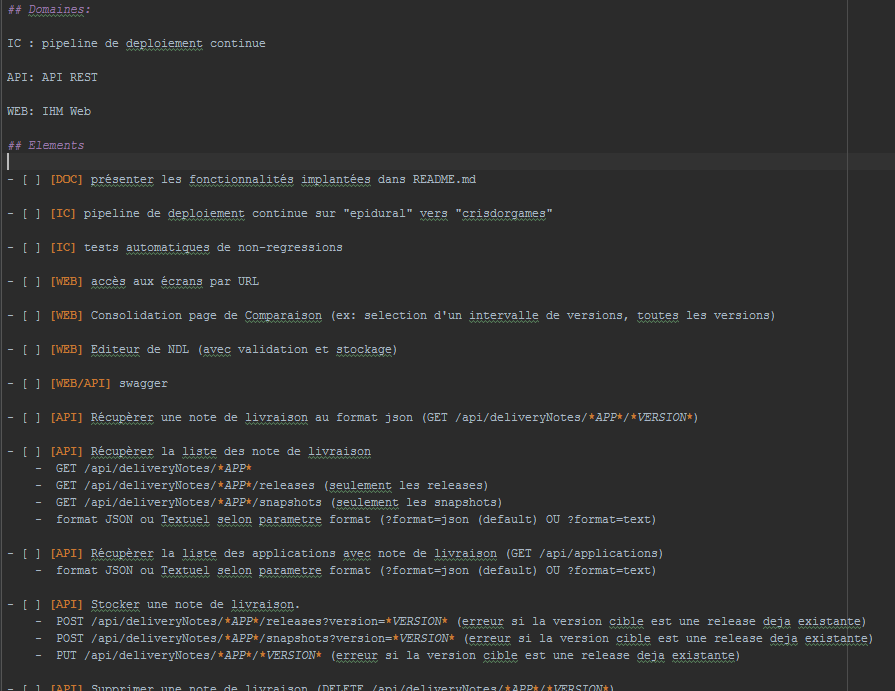
\includegraphics[width=0.7\textwidth]{backlog}
 \caption{Backlog de Dn-Rider}
 \label{fig:backlog}
\end{figure}

Normalement on fait  deux fois par semaine la revue du Kanban pour garder le rythme.
Chaque fois mes tuteurs valident ce que j'ai réalisé et m'aident à planifier les tâches suivantes.

\clearpage
